\documentclass{standalone}

\usepackage[english]{babel} % English language/hyphenation
\usepackage{clock} % Required for generation clock icon
\ClockFrametrue\ClockStyle=3 % Format the clock icons
\usepackage{gensymb} % gives the degree symbol
\usepackage{graphicx} % Required for including pictures
\usepackage{tikz} % Required for drawing custom shapes
\usetikzlibrary{arrows}
\usetikzlibrary{shapes.misc}
\usetikzlibrary{decorations.pathreplacing}

\begin{document}
	\def\glider#1#2#3{
		\begin{scope}[shift={#1}, rotate=#2, scale=#3]
			\fill[black](0,0) -- (1,0) -- (1,1) -- (0,1) -- cycle;
			\fill[black](8/7+0,0) -- (8/7+1,0) -- (8/7+1,1) -- (8/7+0,1) -- cycle;
			\fill[black](16/7+0,0) -- (16/7+1,0) -- (16/7+1,1) -- (16/7+0,1) -- cycle;
			\fill[black](16/7+0,8/7+0) -- (16/7+1,8/7+0) -- (16/7+1,8/7+1) -- (16/7+0,8/7+1) -- cycle;
			\fill[black](8/7+0,16/7+0) -- (8/7+1,16/7+0) -- (8/7+1,16/7+1) -- (8/7+0,16/7+1) -- cycle;
		\end{scope}
	}
	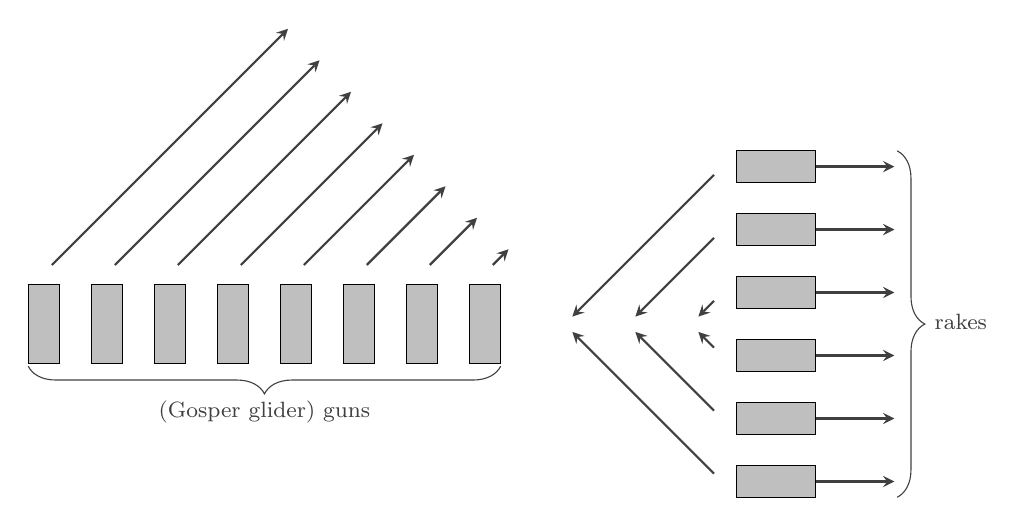
\begin{tikzpicture}%
		% GUNS
		\foreach \x in {0,...,7} \filldraw[color=black,fill=gray!50] (0.8*\x,0) -- (0.8*\x,1) -- (0.4+0.8*\x,1) -- (0.4+0.8*\x,0) -- cycle;
		
		\draw[darkgray,decorate,decoration={brace,amplitude=10pt,mirror},yshift=-1pt]
		(0,0) --node [anchor=north,yshift=-9pt]{\footnotesize (Gosper glider) guns} (6,0);
		
		% GLIDERS from GUNS
		\foreach \x in {0,...,7} \draw[thick,color=darkgray,-stealth] (0.8*\x+0.3,1.25) -- (3.3+0.4*\x,4.25 - 0.4*\x);
		\foreach \x in {0,...,7} \glider{(0.8*\x+0.35,1.04)}{90}{0.08};
		
		% RAKES
		\foreach \x in {0,...,5} \draw[thick,color=darkgray,-stealth] (10,-1.5+0.8*\x) -- (11,-1.5+0.8*\x);
		\foreach \x in {0,...,5} \filldraw[color=black,fill=gray!50] (9,-1.7+0.8*\x) -- (10,-1.7+0.8*\x) -- (10,-1.3+0.8*\x) -- (9,-1.3+0.8*\x) -- cycle;
		\draw[darkgray,decorate,decoration={brace,amplitude=10pt},xshift=1pt]
		(11,2.7) --node [anchor=north,xshift=23pt,yshift=7pt]{\footnotesize rakes} (11,-1.7);
		
		% GLIDERS from RAKES
		\foreach \x in {0,...,2} \draw[thick,color=darkgray,-stealth] (8.71,-1.4+0.8*\x) -- (6.91 + 0.8*\x,0.4);
		\foreach \x in {3,...,5} \draw[thick,color=darkgray,-stealth] (8.71,-1.605+0.8*\x) -- (10.91 - 0.8*\x,0.595);
		\foreach \x in {0,...,2} \glider{(8.94,-1.37+0.8*\x)}{180}{0.08};
		\foreach \x in {3,...,5} \glider{(8.68,-1.37+0.8*\x)}{270}{0.08};
	\end{tikzpicture}
\end{document}